\documentclass[12pt,a4paper]{article}

\input{/home/tabaka/Documents/GitHub/Defs/defs.tex}

\setcounter{zadaniaRozdzial}{6}

\begin{document}
	
	\begin{center}
		\LARGE Karta 6
	\end{center}
	\vspace{1.5cm}
	
	\ZbiorZadanie{Długości boków czworokąta $ABCD$ są równe: $|AB|=2$, $|BC|=3$, $|CD|=4$, $|DA|=5$. Na czworokącie $ABCD$ opisano okrąg. Oblicz długość przekątnej $AC$ tego czworokąta.}
	
	\ZbiorZadanie{Trapez prostokątny $ABCD$ o podstawach $AB$ i $CD$ jest opisany na okręgu. Ramię $BC$ ma długość 10, a ramię $AD$ jest wysokością tego trapezu. Podstawa $AB$ jest 2 razy dłuższa od podstawy $CD$. Oblicz pole tego trapezu.}
	
	\ZbiorZadanie{Odcinek $CD$ jest zawarty w dwusiecznej kąta $ACB$ trójkąta $ABC$. Kąty trójkąta $ABC$ mają miary: $|\angle CAB|=42^\circ$, $|\angle ABC|=78^\circ$. Styczna do okręgu opisanego na tym trójkącie w punkcie $C$ przecina prostą $AB$ w punkcie $E$ (zobacz rysunek).
		
		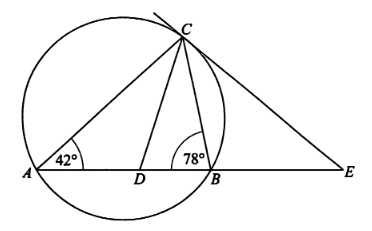
\includegraphics{K_6_1}
		
		Oblicz miary wszystkich kątów trójkąta $CDE$.}
	
	\ZbiorZadanie{Objętość graniastosłupa prawidłowego trójkątnego jest równa $12\sqrt{3}$, a pole powierzchni bocznej tego graniastosłupa jest równe 36. Oblicz sinus kąta, jaki tworzy przekątna ściany bocznej z sąsiednią ścianą boczną.}
	
	\ZbiorZadanie{W ostrosłupie $ABCS$ podstawa $ABC$ jest trójkątem równobocznym o boku długości $a$. Krawędź $AS$ jest prostopadła do płaszczyzny podstawy. Odległość wierzchołka $A$ od ściany $BCS$ jest równa $d$. Wyznacz objętość tego ostrosłupa.}
	
	\ZbiorZadanie{Rzucamy cztery razy symetryczną sześcienną kostką do gry. Oblicz prawdopodobieństwo zdarzenia polegającego na tym, że iloczyn liczb oczek uzyskanych we wszystkich czterech rzutach będzie równy 60.}
	
	
	
\end{document}